\documentclass[a4paper]{article}
\addtolength{\hoffset}{-2.25cm}
\addtolength{\textwidth}{4.5cm}
\addtolength{\voffset}{-3.25cm}
\addtolength{\textheight}{5cm}
\setlength{\parskip}{0pt}
\setlength{\parindent}{0in}

\usepackage[square,sort,comma,numbers]{natbib}
\usepackage{blindtext} % Package to generate dummy text
\usepackage{charter} % Use the Charter font
\usepackage[utf8]{inputenc} % Use UTF-8 encoding
\usepackage{microtype} % Slightly tweak font spacing for aesthetics
\usepackage{amsthm, amsmath, amssymb} % Mathematical typesetting
\usepackage{float} % Improved interface for floating objects
\usepackage{hyperref} % For hyperlinks in the PDF
\usepackage{graphicx, multicol} % Enhanced support for graphics
\usepackage{xcolor} % Driver-independent color extensions
\usepackage{pseudocode} % Environment for specifying algorithms in a natural way
\usepackage[mmddyy]{datetime} % Uses YEAR-MONTH-DAY format for dates

\usepackage{fancyhdr} % Headers and footers
\pagestyle{fancy} % All pages have headers and footers
\fancyhead{}\renewcommand{\headrulewidth}{0pt} % Blank out the default header
\fancyfoot[L]{} % Custom footer text
\fancyfoot[C]{} % Custom footer text
\fancyfoot[R]{\thepage} % Custom footer text
\newcommand{\note}[1]{\marginpar{\scriptsize \textcolor{red}{#1}}} % Enables comments in red on margin

\DeclareMathOperator*{\argmin}{arg\,min}

%----------------------------------------------------------------------------------------

\newcommand{\yourname}{Balthazar Neveu}
\newcommand{\youremail}{balthazarneveu@gmail.com}
\newcommand{\assignmentnumber}{5}

\begin{document}

\fancyhead[C]{}
\hrule \medskip
\begin{minipage}{0.295\textwidth} 
\raggedright
\footnotesize
\yourname \hfill\\
\youremail
\end{minipage}
\begin{minipage}{0.4\textwidth} 
\centering 
\large 
Lab session \# \assignmentnumber\\ 
\normalsize 
ALTEGRAD 2023\\ 
\end{minipage}
\begin{minipage}{0.295\textwidth} 
\raggedleft
\today\hfill\\
\end{minipage}
\medskip\hrule 
\bigskip


\section*{Code}
For part 1, I set up a 4 CPU TensorDock remote machine to avoid working on my local machine.
This took some time. Pre-requisite setup.sh \& download\_models.sh .

More info:
\href{https://github.com/balthazarneveu/MVA23_ALTEGRAD/#readme}{MVA ALTEGRAD Balthazar Neveu on Github}

\section{Unsupervised node embeddings using Deepwalk}

We're trying to construct meaningful for a graph made of crawled french websites.

\begin{itemize}
    \item Number of nodes: 33226 . Each node is a website link.
    \item Number of edges: 354529 . Edges means the presence of hyperlinks between 2 websites.
    \item Dimension of embeddings of Word2Vec: 128
    \item Random walk length = 20
    \item At each node, $n_{walks}=10$ will be pre-stored.
\end{itemize}

\subsection*{Task 1 \& 2: Details on random walks sampling implementations}
Unexpectedly, initial naïve implementation took way too much time. 
Profiling led me to spot two bottlenecks:
\begin{itemize}
    \item I should not use \textit{np.random.choice} but rather \textit{random.randint} 
    to sample the next node in the walk
among neighbors.
    \item In addition, I used a dictionary to pre-store the neighbors instead of using the remove redundant calls to \textit{list(G.neighbors(node))}
    \item In this dataset, nodes are not indexes (e.g. integers) but string (hyperlinks).
    I tried to relabel to ints but it didn't really sped up and addressing the first two points was enough.
\end{itemize}

\begin{verbatim}
# Create a mapping from strings to integers
node_mapping = {node: i for i, node in enumerate(G.nodes())}

# Create a reverse mapping if you need to convert back to strings later
reverse_mapping = {i: node for node, i in node_mapping.items()}
G_int = nx.relabel_nodes(G, node_mapping)
\end{verbatim}

\subsection*{Task 4 : Node embdeddings visualization}
Refer to  \ref{fig:node_embeddings}
\begin{figure}[ht]
    \centering
    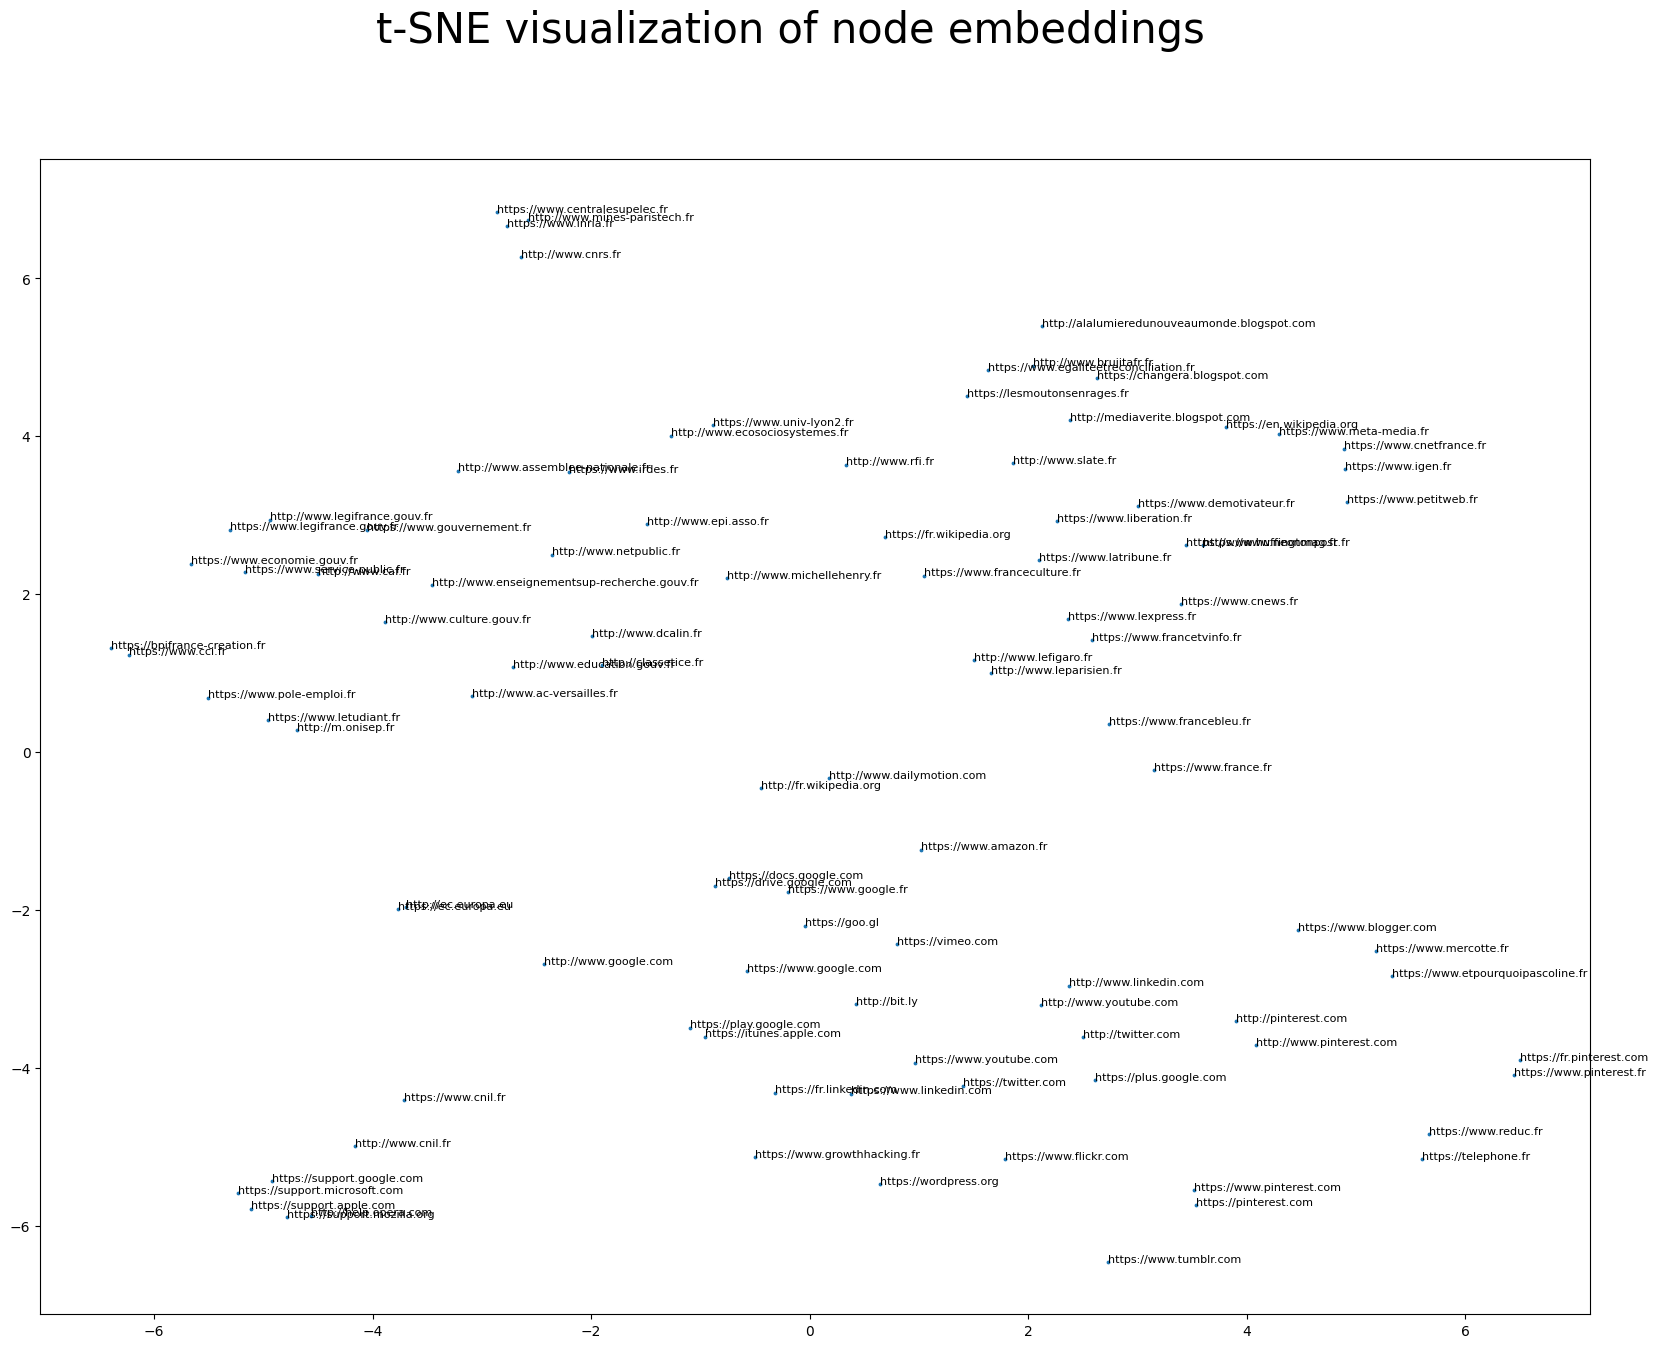
\includegraphics[width=1.\textwidth]{figures/tSNE_node_embeddings.png}
    \caption{t-SNE is used on the high (128) dimensional node embeddings to reduce dimensionality to 2D coordinates,
    which allows visualization of a few samples (here $n=100$)}
    \label{fig:node_embeddings}
\end{figure}

\subsection*{Question 1}


\subsection*{Nodes within Connected Components}
For nodes within each $K_2$ component, we expect a high cosine similarity in their embeddings. \\
In a $K_2$ graph, the only possible walks are between the two connected nodes. \\
The DeepWalk algorithm, which relies on these walks to generate embeddings,
will frequently observe these two nodes in proximity. 
Consequently, their vector embeddings will be very similar,
reflecting their direct and exclusive connection in the graph.

\subsection*{Nodes in Different Connected Components}
In contrast, nodes in different $K_2$ components are expected to exhibit lower cosine similarity in their embeddings. \\
Each $K_2$ is an isolated connected component, 
implying that random walks within one $K_2$ component do not include nodes from another $K_2$ component. \\
As a result, the embeddings generated by DeepWalk will capture this lack of relation in the graph structure, 
leading to lower similarity in the vector space for nodes from different components.

\section{Node classification}
\subsection*{Task 6: Classification of Zachary's karate club - 100\% accuracy}

\begin{figure}[ht]
    \centering
    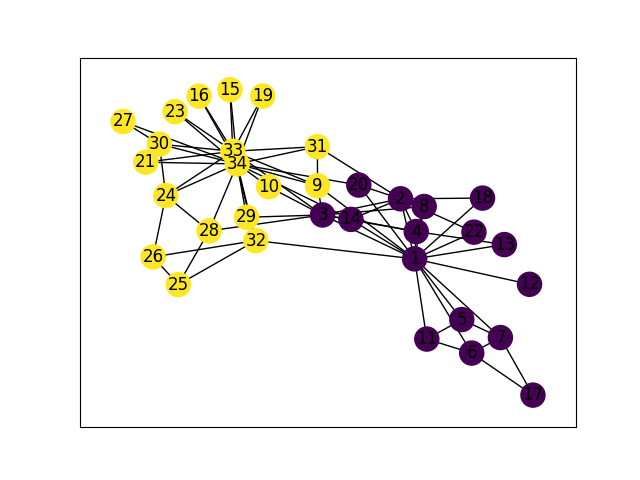
\includegraphics[width=1.\textwidth]{figures/labeled_karate_graph.png}
    \caption{Karate graph with 2 labels}
    \label{fig:karate_labeled}
\end{figure}


\begin{verbatim}
Epoch: 100 loss_train: 0.0640 acc_train: 1.0000 time: 0.0025s
\end{verbatim}

\bibliographystyle{plain}
\bibliography{references} % citation records are in the references.bib document

\end{document}